\documentclass[a4paper]{article}

%% Language and font encodings
\usepackage[french]{babel}
\usepackage[utf8x]{inputenc}
\usepackage[T1]{fontenc}

%% Sets page size and margins
\usepackage[a4paper,top=3cm,bottom=3cm,left=2cm,right=2cm,marginparwidth=2cm]{geometry}

%% Useful packages
\usepackage{amsmath}
\usepackage{graphicx}
\usepackage[colorinlistoftodos]{todonotes}
\usepackage[colorlinks=true, allcolors=black]{hyperref}
\usepackage{fourier-orns}
\usepackage{titlesec}
\usepackage{fancyhdr}
\usepackage{fancyvrb}
\usepackage{float}
\pagestyle{fancy} 
\setcounter{tocdepth}{5}


%% Tikz stuff
\usepackage{tikz}
\usetikzlibrary{calc, arrows}
\tikzstyle{incolore} = [rectangle, rounded corners, draw=black, minimum height=1cm, minimum width=3cm, text width=3cm, text centered]



\usepackage{libertine}
\newcommand{\hsp}{\hspace{20pt}}
\newcommand{\HRule}{\rule{\linewidth}{0.5mm}}





\renewcommand{\headrulewidth}{1pt}
\fancyhead[C]{} 
\fancyhead[L]{}
\fancyhead[R]{\footnotesize{\leftmark}}

\renewcommand{\footrulewidth}{1pt}
\fancyfoot[C]{} 
\fancyhead[L]{}
\fancyfoot[R]{\thepage}

\definecolor{Zgris}{rgb}{0.87,0.85,0.85}

\usepackage{eso-pic,graphicx}
\usepackage{xcolor}
\newcommand{\bgimg}[1]{
\AddToShipoutPicture
   {
      \put(\LenToUnit{0 cm},\LenToUnit{0 cm})
      {
            \includegraphics[width=\paperwidth,height=\paperheight]{#1} 
      }
   }
}
\begin{document}




%%\bgimg{Image_15.jpg}

















\begin{titlepage}
    \begin{sffamily}
        \begin{center}
            
\includegraphics[width=5cm]{images/LogoHenallux.PNG}~\\[1.5cm]
            \textsc{\Large Rapport de laboratoire}\\[1.5cm]

            % Title
            \HRule \\[0.4cm]
            { \huge \bfseries Cinquième laboratoire : RS232\\[0.4cm] }
            \HRule \\[2cm]

            % Author and supervisor
            \begin{minipage}{0.4\textwidth}
                \begin{flushleft} \large
                    Roumache Grégoire\\
                    Sénéchal Julien\\
                    Robert Alexandre\\
                    Wallemme Maxime\\
                    Kenmeugne Lionel\\
                    Didion Charles
                \end{flushleft}
            \end{minipage}
            \begin{minipage}{0.55\textwidth}
                \begin{flushright} \large
                    Laboratoire de sciences appliquées à l'informatique\\
                    Sécurité des systèmes, technologie de l'informatique\\
                    Hénallux\\
                    Première année, groupe H \\
                    Année académique 2019-2020\\
                \end{flushright}
            \end{minipage}
            \vfill

            % Bottom of the page
            {\large 26 Mars 2020}
        \end{center}
    \end{sffamily}
\end{titlepage}







\let\cleardoublepage\clearpage















\section{Introduction}





Lors de cette manipulation, nous avons l'occasion de pouvoir découvrir le fonctionnement des ports de communication qu'on tous nos ordinateurs.\\
Tout d'abord, nous verrons le principe de fonctionnement du port série d'un PC. Ensuite, nous verrons plus en détails la communication série asynchrone (\emph{RS232}) : \emph{protocole - trame – signaux}. Puis, quelques explications sur le code ASCII. Enfin, nous pourrons voir que nous apporte comme informations la manipulation et quel sont les observations et conclusions  que nous pourrons alors en tirer.















\section{Rappels théoriques}










\subsection{Principe et fonctionnement d’un port série PC}





Pour y voir plus clair, commençons par se renseigner sur ce que veut dire le titre de la manipulation, à savoir "RS-232". \\
RS-232 est en fait une norme de standardisation des câble séries. Sa période d’utilisation pourrait être définie de 1981 à 2005, bien qu’encore utilisée à l’heure actuelle sur certains PC (DB-9). Plus loin dans la manip, dans le logiciel, on parlera de port "COM1". Même principe, est-ce que ce nom a une signification ? Eh bien oui, il y en a une le COM1 similaire au COM2 désigne un type de système d’exploitation le plus ancien MS-DOS (COM1) et le port Windows plus récent (COM2).

Pour terminer cette partie de recherche d’information, il faut préciser qu’à l’heure actuel ce port n’est presque plus utilisé, au profit du port USB.





Ce câble est d’une grande robustesse et possède deux extrémités différentes. Le connecteur mâle (DB-25) se branche du côté du PC : "relié à la carte mère". Il possède entre 9 et 25 broches.

\begin{figure}[H]
    \centering
    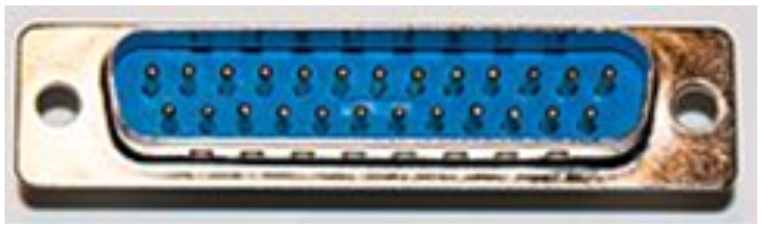
\includegraphics[width=0.5\textwidth]{images/ConnecteurMaleDB25.PNG}
    \caption{Connecteur mâle DB-25}
    \label{fig:ConnecteurMaleDB25}
\end{figure}

Le connecteur femelle (BD-25) se branche du coté DCE (l’équipement de communication de données). Il s’agit de tout appareil qui achemine les informations vers/depuis un réseau. Par exemple un Modem ou un switch.

\begin{figure}[H]
    \centering
    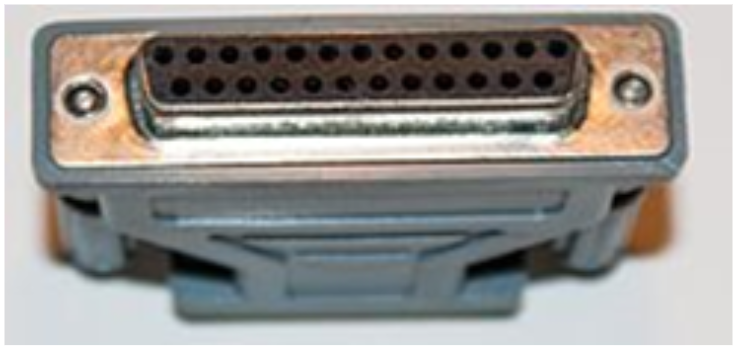
\includegraphics[width=0.5\textwidth]{images/ConnecteurFemelleBD25.PNG}
    \caption{Connecteur femelle BD-25}
    \label{fig:ConnecteurFemelleBD25}
\end{figure}

Il faut savoir que toute une série de paramètres peuvent être définis mais il existe des protocoles par défaut. Le débit, le découpage en trame, le codage sont, par exemple, liés à un protocole disponible par défaut à UART relativement conventionnel. Il est modifiable via logiciel et visualisable pour exemple dans la manipulation via le programme port COM.

Les échanges de données se font de manière asynchrone. En d’autres termes, il n’est pas nécessaire de suivre le battement d’une horloge et les données peuvent être envoyer à un rythme qui n’est pas toujours le même. Pour délimiter la fin et le début du signal, il y a un bit de début (START) et un bit de fin (STOP). Les bits de contrôles prennent environ 20 \%  de la bande passante.










\subsection{Description de la communication série asynchrone : protocole - trame – signaux}





La communication série permet à divers systèmes numériques de se transmettre de l’information. Elle est asynchrone ce qui signifie qu’elle n’est basée sur aucune fréquence d’horloge. 

Concernant le protocole d’échange, la communication commence lors de l’envoi d’un "bit start" permettant au récepteur de savoir qu’une nouvelle donnée va arriver et connaître la vitesse à laquelle les données vont suivre. Pour terminer la transmission, on envoie un "bit stop" pour permettre au récepteur de savoir qu’il ne recevra plus de données après ça. Il y a également un bit de parité envoyé durant la transmission afin de vérifier les erreurs. Le bit start est généralement un bit à 0, le bit de parité lui est à 1 ou 0 et le bit stop est généralement à 1, 1 et demi ou 2 afin de ne pas le confondre avec un bit de départ.

Le signal transmis est donc un signal binaire, la durée d’émission de chaque bit est la même.

La trame du signal est donc représentée comme sur la figure \ref{fig:RepresentationTrameSignal}.

\begin{figure}[H]
    \centering
    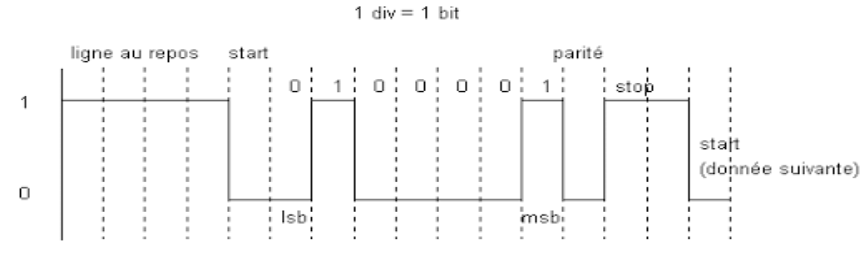
\includegraphics[width=0.85\textwidth]{images/RepresentationTrameSignal.PNG}
    \caption{Représentation de la trame du signal}
    \label{fig:RepresentationTrameSignal}
\end{figure}

Le signal est tout d’abord au repos, puis un bit de start est envoyé au récepteur, donnant ainsi l’informations que des données vont suivre composée d’un bit de parité pour vérifier les éventuelles erreurs. Et cette communication est terminée par un bit stop.










\subsection{Code ASCII}





Le code ASCII (American Standard Code for Information Interchange) est une norme de codage des caractères sous un format binaire. Il contient 127 caractères, les caractères peuvent donc être codés sur 7 bits même si on utilise souvent le 8 bits à cause de l’architecture des ordinateurs qui utilise souvent des octets. Comme il a été développé pour la langue anglaise, il n’est pas approprié pour représenter les caractères qui sont peu fréquents en anglais comme les accents. Les langues possédant un alphabet différent de l’alphabet latin ou utilisant des accents doivent donc utiliser d’autres codages de caractères. Le code ASCII est cependant très utilisé de par l’influence de l’anglais sur l’informatique.















\section{Manipulation pratique}





Dans cette manipulation, nous devions utiliser le matériel suivant:
\begin{itemize}
    \item un oscilloscope qui sert à visualiser les signaux ;
    \item un multimètre pour mesurer les tensions dans le boîtier de visualisation RS232 ;
    \item un câble de liaison série pour connecter le PC au boîtier de visualisation ;
    \item un boîtier de visualisation RS232 pour décoder des messages envoyés avec le protocole RS232 depuis l’ordinateur ;
    \item un logiciel de transmission.    
\end{itemize}
Pour commencer, on doit mesurer les tensions fournies par le boîtier de visualisation quand on envoie un 1 logique et quand on envoie un 0 logique. Ensuite, on doit envoyer la valeur 521 en texte au format ASCII depuis l’ordinateur vers le boîtier de visualisation. Ce message s’affiche normalement dans une fenêtre du boîtier de visualisation après "Texte ou nombre reçu". Nous devons maintenant mesurer le "baud rate" du message à l’aide de l’oscilloscope, c’est à dire que nous devons mesurer la rapidité de modulation du signal. Pour le faire, il faut mesurer la durée de l’élément le plus court sur l’oscilloscope. Autrement dit, nous devons mesurer la durée d’un bit.















\section{Conclusion}





En conclusion, le port COM est une ancienne technologie, mais elle était déjà bien pensée. Son connecteur 25 broches permet à une série de paramètres, tel que le protocole de segmentation, d’être modifié. Grace a l’utilisation de bits de début et de fin ainsi que d’un bit de parité le tout à travers un signal en série. C’est un port robuste adapté à l’utilisation par les particuliers des années 80.















\newpage \tableofcontents \listoffigures
\begin{thebibliography}{9}

\bibitem{1} https://www.commentcamarche.net/contents/770-port-serie-et-port-parallele
\bibitem{2} https://sitelec.org/cours/abati/rs232.htm
\bibitem{3} https://www.aurel32.net/elec/port\_serie.php

\bibitem{4} http://www.groupeisf.net/reseaux\_informatiques/reseaux\_et\_telecommunications/reseaux/liaisons\_series/\\
rs232/index\_fichiers/rs232.gif
\bibitem{5} https://www.electronique-mixte.fr/wp-content/uploads/2018/07/Formation-Interface-communication-6.pdf
\bibitem{6} https://www.youtube.com/watch?v=qYKCOauFzsk\&t=280s
\bibitem{7} https://les-electroniciens.com/sites/default/files/cours/cours-communications-asynchrones.i2621.v080.pdf
\bibitem{8} http://math.univ-lyon1.fr/irem/Formation\_ISN/formation\_rs232/tp/ISN\_TP\_rs232\_eleve\_correction.pdf

\bibitem{9} https://fr.wikipedia.org/wiki/American\_Standard\_Code\_for\_Information\_Interchange
\bibitem{10} https://www.commentcamarche.net/contents/93-code-ascii
\end{thebibliography}














\end{document}
